\chapter{Implementation}
\section{}
\section{Metadata storage and discovery}
\subsection{Release blocks}
Releases are objects that represent an audio release produced by one or more artists. For example this is an album, an EP, a single, or a podcast. Release objects are stored on the TrustChain, and are exchanged between peers that are part of the MusicCommunity (see \ref{sec:music-community}). These objects are structured as shown in \ref{fig:release-implementation}. The \textit{magnet} property contains a magnet link which holds all additional information about the contents of the Release, such as the torrent file list, size and tracker URLs. The \textit{publisher} property contains the public key of a Bitcoin wallet which is owned by the creator of the Release. This public key is an identity of the owner of the record (either the artist, band or label) and can be seen as a proof of the identity of an artist or collaboration between them. 
% When a torrent is created from a local file list, the TorrentInfoName value is established. 
\begin{figure}
    \minipage{0.2\textwidth}
        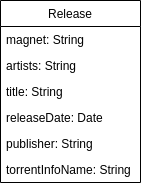
\includegraphics[width=\linewidth]{implementation/release-implementation.png}
        \caption{Release blocks structure as seen on TrustChain}
        \label{fig:release-implementation}
    \endminipage\hfill
    \minipage{0.3\textwidth}
        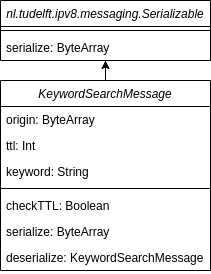
\includegraphics[width=\linewidth]{implementation/keyword-search-message.png}
        \caption{KeywordSearchMessage object sent over IPv8 in MusicCommunity}
        \label{fig:keyword-search-message}
    \endminipage\hfill
    \minipage{0.5\textwidth}
    \endminipage
\end{figure}
\subsection{Searching}
The MusicCommunity extends the TrustChainCommunity with additional methods \textit{performRemoteKeywordSearch} and \textit{onKeywordSearch} which allows peers to search for content using keywords, both locally and remotely. These methods test each \textit{title}, \textit{artists} and \textit{date} field of each Release block against a \verb|contain(keyword)| filter. This means: if the keyword is contained in one of those values, it is added to the results.

When the user performs a search, the local database is filtered first to find matches. If there are less than \(x\) results, the device sends a KeywordSearchMessage (see X) to a maximum of \(P\) known peers in the MusicCommunity. This asks neighbours to inspect their local database to find matches for the same query. Upon receival, the peer subtracts 1 from the time to live (TTL) field. If the peer finds a match, it sends the corresponding TrustChain block directly back to the original asker, appointed by the \textit{origin} field. This contains the IPv8 \textit{peer ID}~\citep{mattskala2020} of the peer that initiated the search. Otherwise, if the time to live (TTL) is more than 1, the peer forwards this KeywordSearchMessage (see \ref{fig:keyword-search-message)}) to other peers. Our keyword search is implemented with default values of \(T=1, P=20, x=5\) (where \(T\) is the TTL).

\section{Networking}
\subsection{Torrent creation and sharing}
\label{sec:torrent-creation}
We use the JLibtorrent implementation by Frostwire\footnote{\url{https://github.com/frostwire/frostwire-jlibtorrent}} of BitTorrent to interact with BitTorrent peers. In our application, a user can select local audio tracks, after which a torrent file is generated with the corresponding metadata. Alternatively, the user can paste a preexisting torrent magnet link to use for the Release block, as shown in \ref{fig:select-tracks}. The creation of torrents by the app happens as follows. First, the user presses the \textit{Select Local Audio} button in the release creation dialog (see \ref{fig:submit-release-dialog}). Afterwards, the user selects one or more tracks to add (see \ref{fig:select-tracks}). In the background this creates a torrent file (using the Ttorrent library\footnote{\url{http://mpetazzoni.github.io/ttorrent/}}), which is stored on the mobile device, and added to the ContentSeeder (see \ref{sec:content-seeder}). Finally, by using the computed infohash and file list, the magnet link of the torrent file is created and added to the \textit{magnet} field of the Release block.

By default, the torrents created using MusicDAO are marked as `trackerless' meaning that torrent peers are found using a distributed hash table~\citep{dht2019} (specifically, mainline DHT\footnote{\url{https://www.libtorrent.org/dht_extensions.html}})instead of centralized trackers. This is to keep the app independent on connectivity on trackers and pushes towards a fully distributed system.

In addition, the app enables the local peer discovery (LPD)~\citep{bittorrentbep142015} functionality of BitTorrent. This allows for finding peers and transmitting torrent pieces over local area network. This results in higher transmission speed and lower latency for content that is stored in the cache of devices nearby. For example, if device A is looking for track X, and device B has this track cached and is active on the same local area network, this track can be found and buffered quickly from A.
\begin{figure}
    \minipage{0.3\textwidth}
        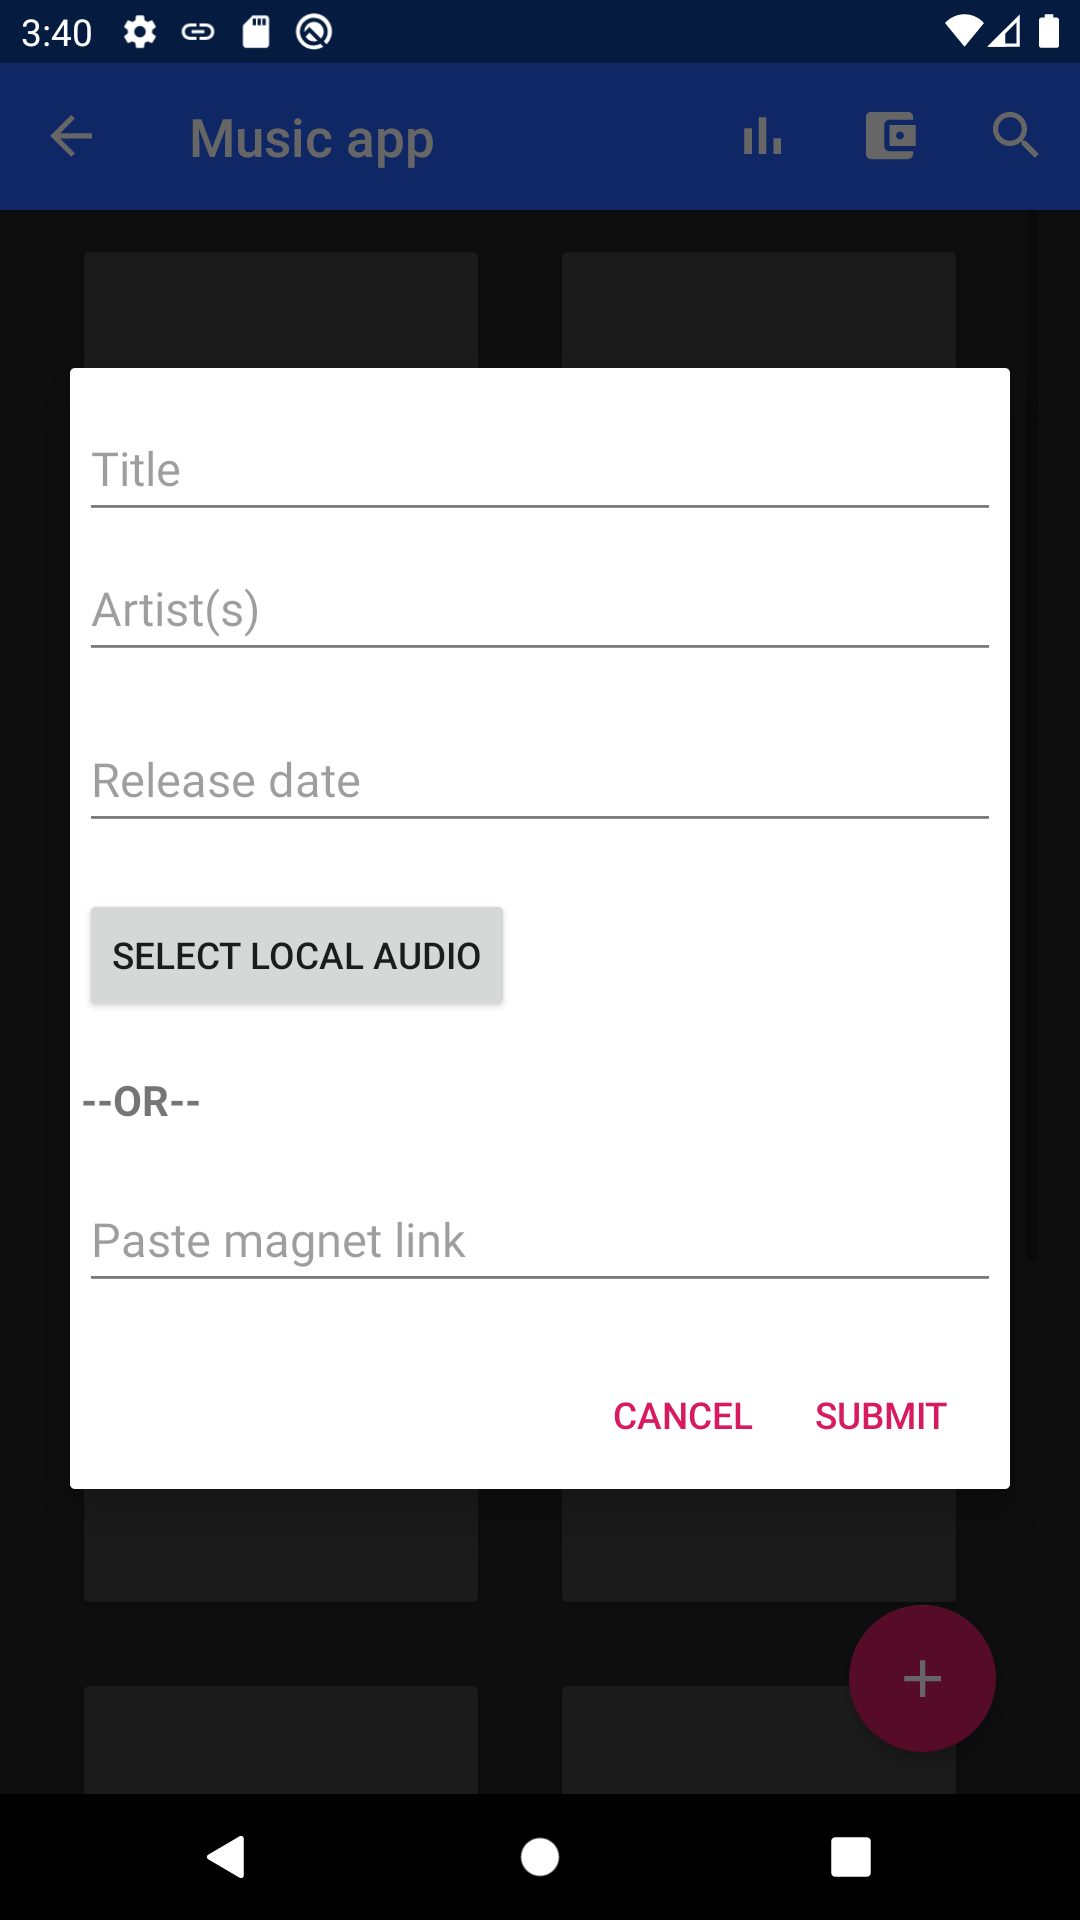
\includegraphics[width=\linewidth]{implementation/screenshot-select-tracks.png}
        \caption{Dialog for creating and publishing a new Release}
        \label{fig:submit-release-dialog}
    \endminipage\hfill
    \minipage{0.3\textwidth}
        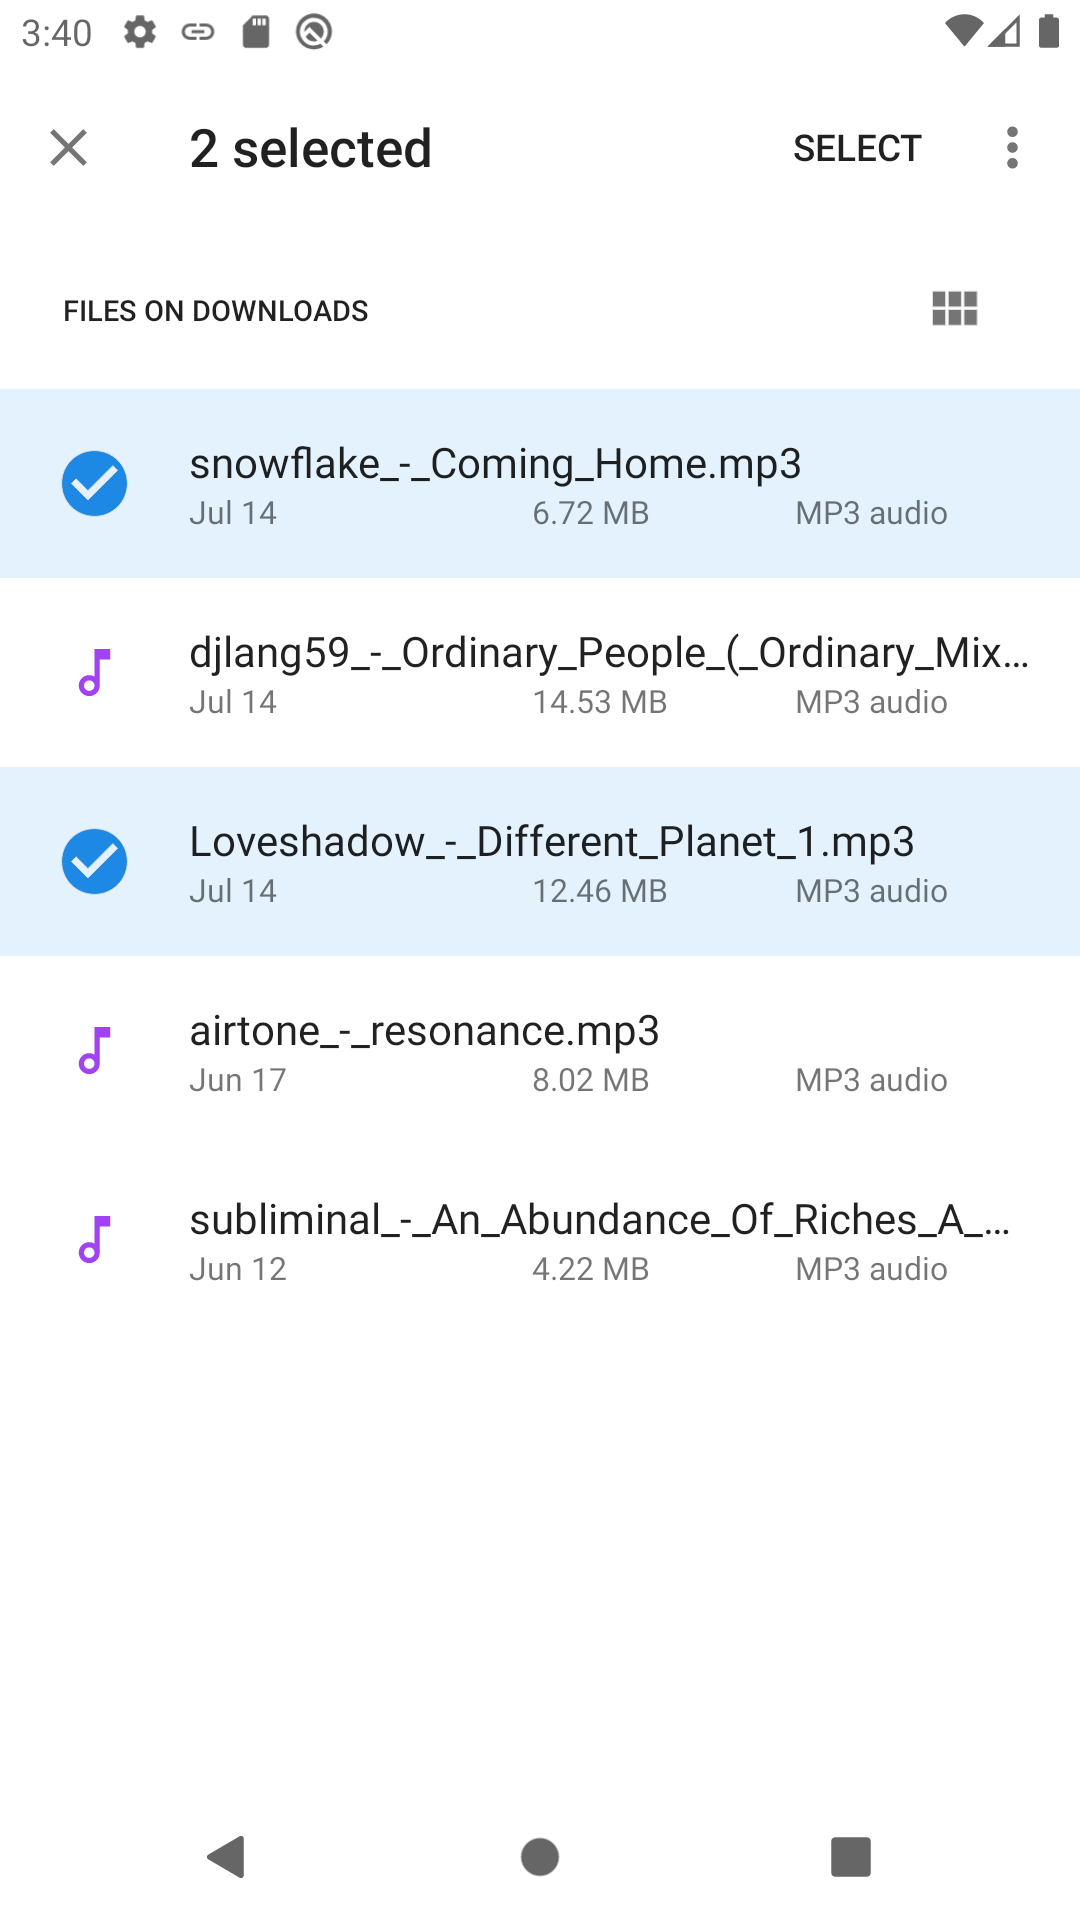
\includegraphics[width=\linewidth]{implementation/screenshot-submit-release.png}
        \caption{Selecting local tracks for creating a new Release}
        \label{fig:select-tracks}
    \endminipage\hfill
    \minipage{0.3\textwidth}
    \endminipage
\end{figure}
\subsection{Content sharing}
Seeding of content is implemented using a simple continuous mechanism. On startup, the ContentSeeder class (see X) spawns a background thread which iteratively scans all torrent files in the local cache directory of the app. There is an upper threshold for how many torrents are selected for seeding. This threshold is currently set to \(X=10\). The ContentSeeder uses a last-in-first-out heuristic: the top \(X\) most recent created/received torrent files are seeded.

\section{Music Player and Streaming}
Playing music is implemented using ExoPlayer 2.10\footnote{\url{https://github.com/google/ExoPlayer}}. This music player library is suitable as it allows for playing tracks that are partially loaded, which allows for streaming.
\subsection{Priority handling}
To provide the user with selected content as soon as possible, we implemented a system which sets priorities on certain tracks and torrent chunks. This uses the piece priorities system in libtorrent, which range from the integers 1 (normal) to 7 (highest) (see libtorrent Manual\footnote{\url{https://www.libtorrent.org/manual-ref.html\#file-format}}). When a user selects a track, this track is given a high \textit{file\_priority} of 5. This is a higher priority than that of other files, so JLibtorrent asks actively for peers who have this file. In addition, the first 5  pieces of the selected track are given a \textit{piece\_priority} of 7, so that the first seconds of the track are buffered quickly and the user can start streaming early.
\subsection{Seeking and buffering}
The music player tries to play the track once a satisfactory portion is loaded. This is implemented as follows. Upon seeking a part of the track, the torrent piece index on which the cursor is located is calculated. Afterwards, the piece at this index and the 5 consequent pieces are given a \textbf{piece\_priority} of 7, which is higher than the other pieces. Once at least 2000 ms from the cursor is buffered, the music player starts playing the track. This way the user can start playing the portion of the track they are most interested in quickly.
\section{Donations and payments}
\subsection{Bitcoin RegTest network}
We created a public Bitcoin RegTest environment\footnote{\url{https://developer.bitcoin.org/examples/testing.html\#regtest-mode}} to test peer-to-peer Bitcoin donations and payments. This creates a new `clean slate' Bitcoin blockchain and allows for full control over the chain and miners. This enables a test environment that is useful for experiments, as we can tweak the block generation speed and read all transactions registered on the closed-off blockchain.
\label{sec:regtest-network-impl}
\section{Interface}
\subsection{Playlist overview}
The playlist overview screen, as shown in \ref{fig:screenshot-home} is the screen that is first shown upon starting the MusicDAO. Here the user is presented a list of playlists, loaded from their local database TrustChain instance. Currently, each Playlists fragment corresponds to exactly one Release block (see ref). In the background runs an iterative process which checks whether new playlist content is found, and re-renders the view if necessary. The playlists are sorted on their torrent swarm health in ascending order. 
\begin{figure}
    \minipage{0.3\textwidth}
        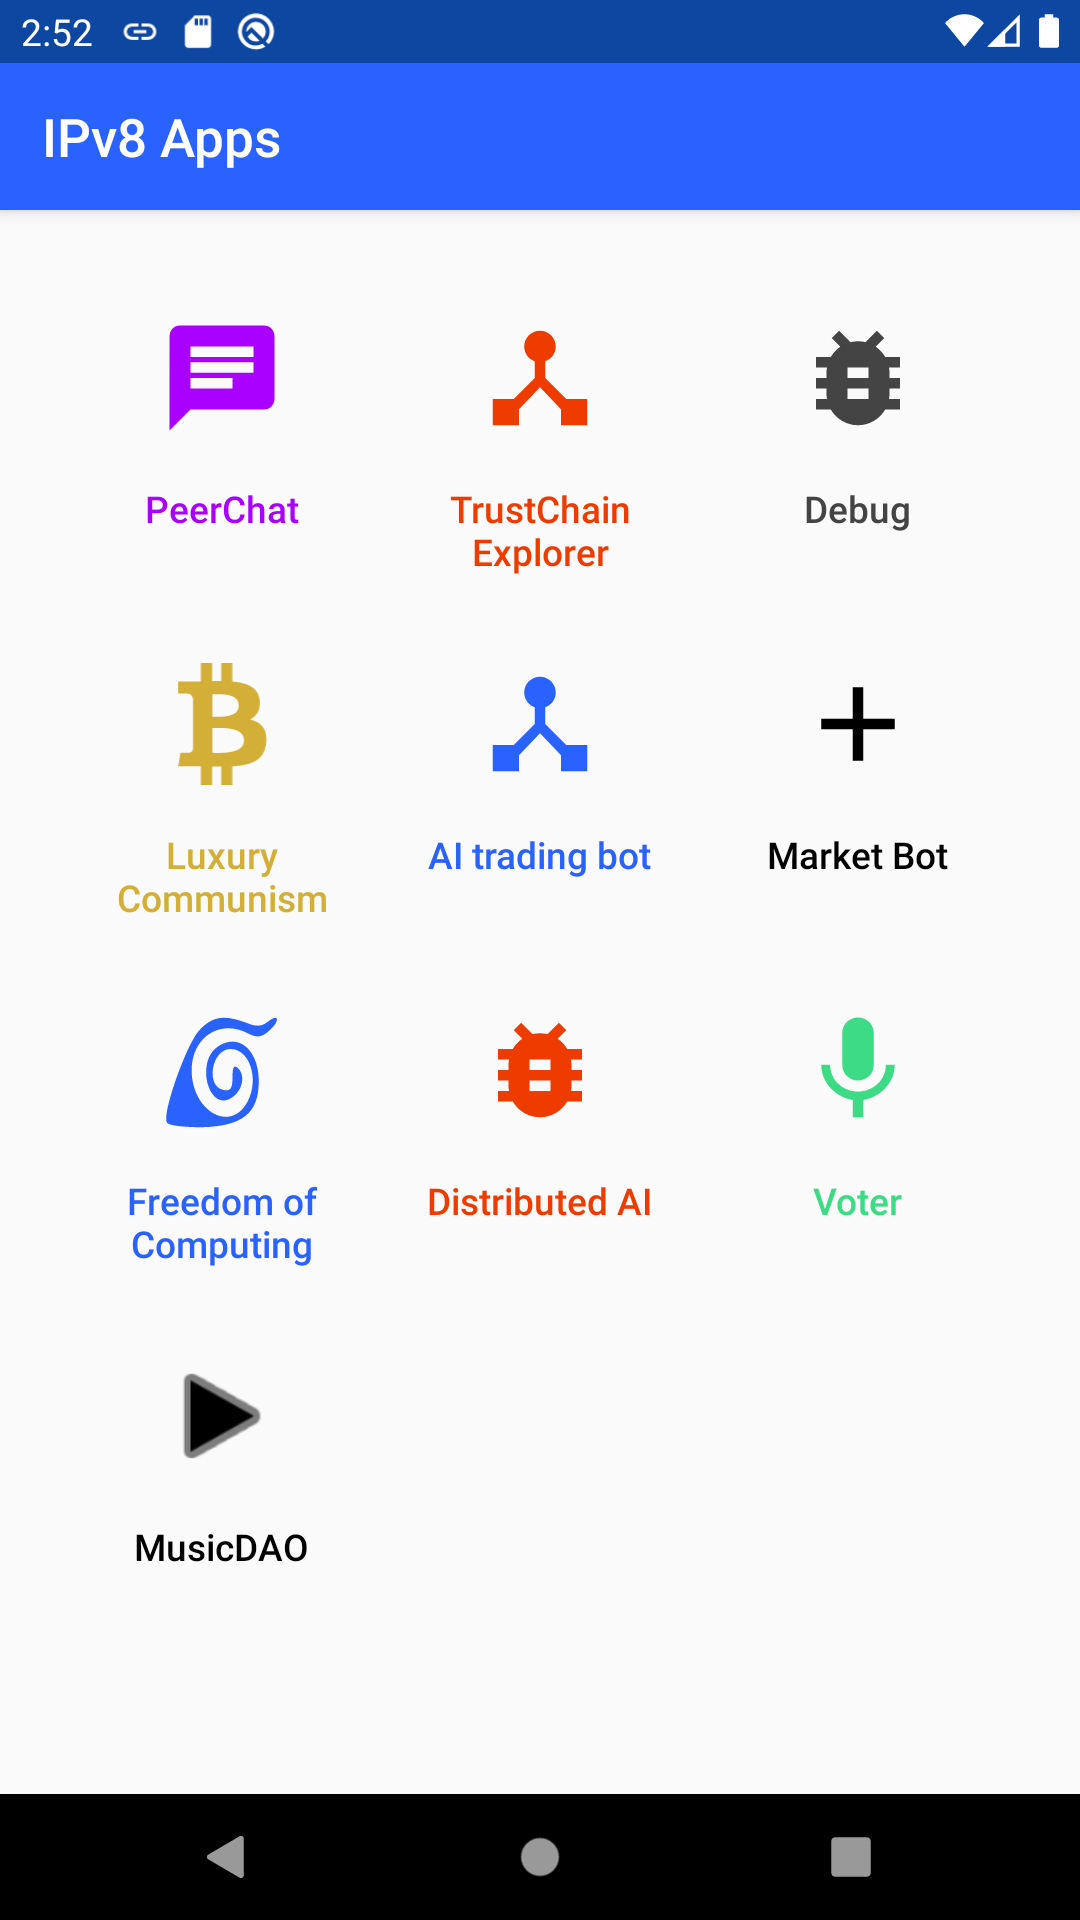
\includegraphics[width=1\linewidth]{implementation/screenshot-superapp.png}
        \caption{The app is integrated as a mini-app in the IPv8 Superapp catalog}
        \label{fig:screenshot-superapp}
    \endminipage\hfill
    \minipage{0.3\textwidth}
        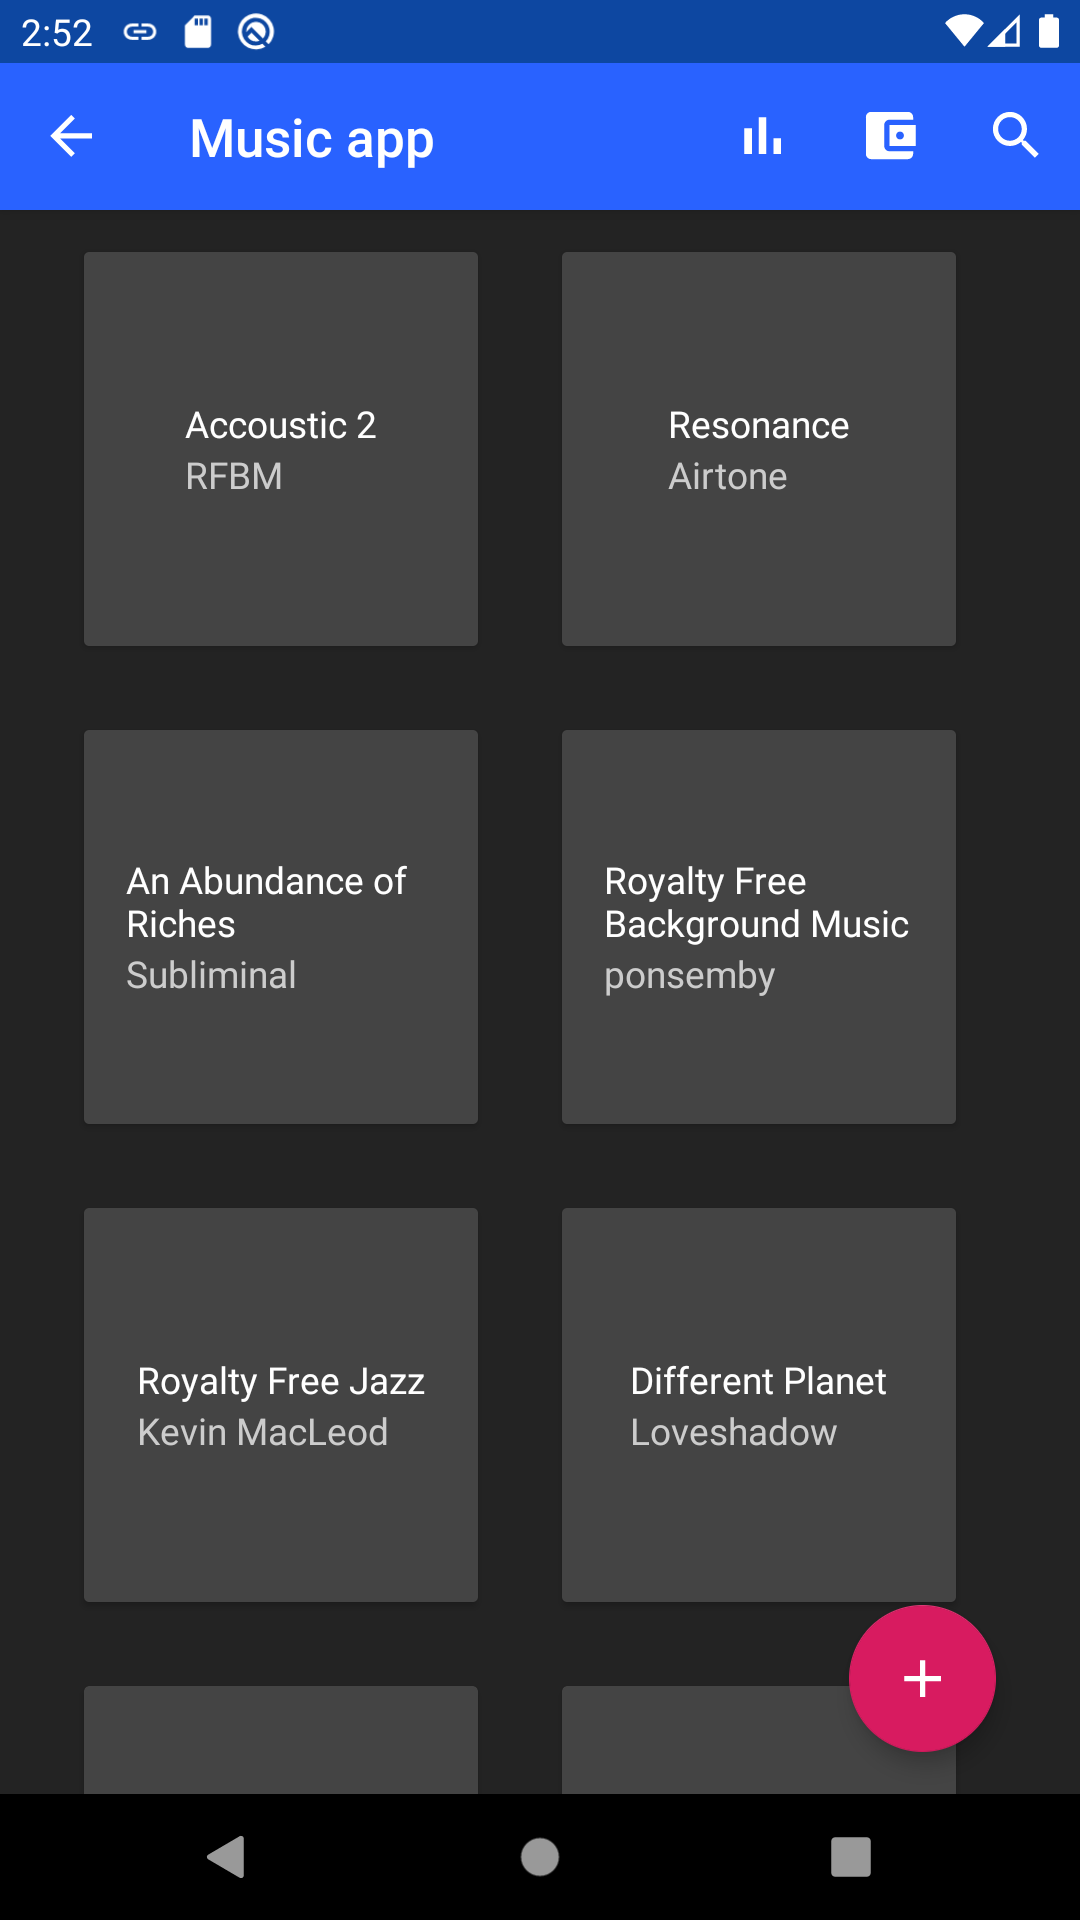
\includegraphics[width=1\linewidth]{implementation/screenshot-home.png}
        \caption{The playlist overview screen, which is the entrance screen}
        \label{fig:screenshot-home}
    \endminipage\hfill
    \minipage{0.3\textwidth}
        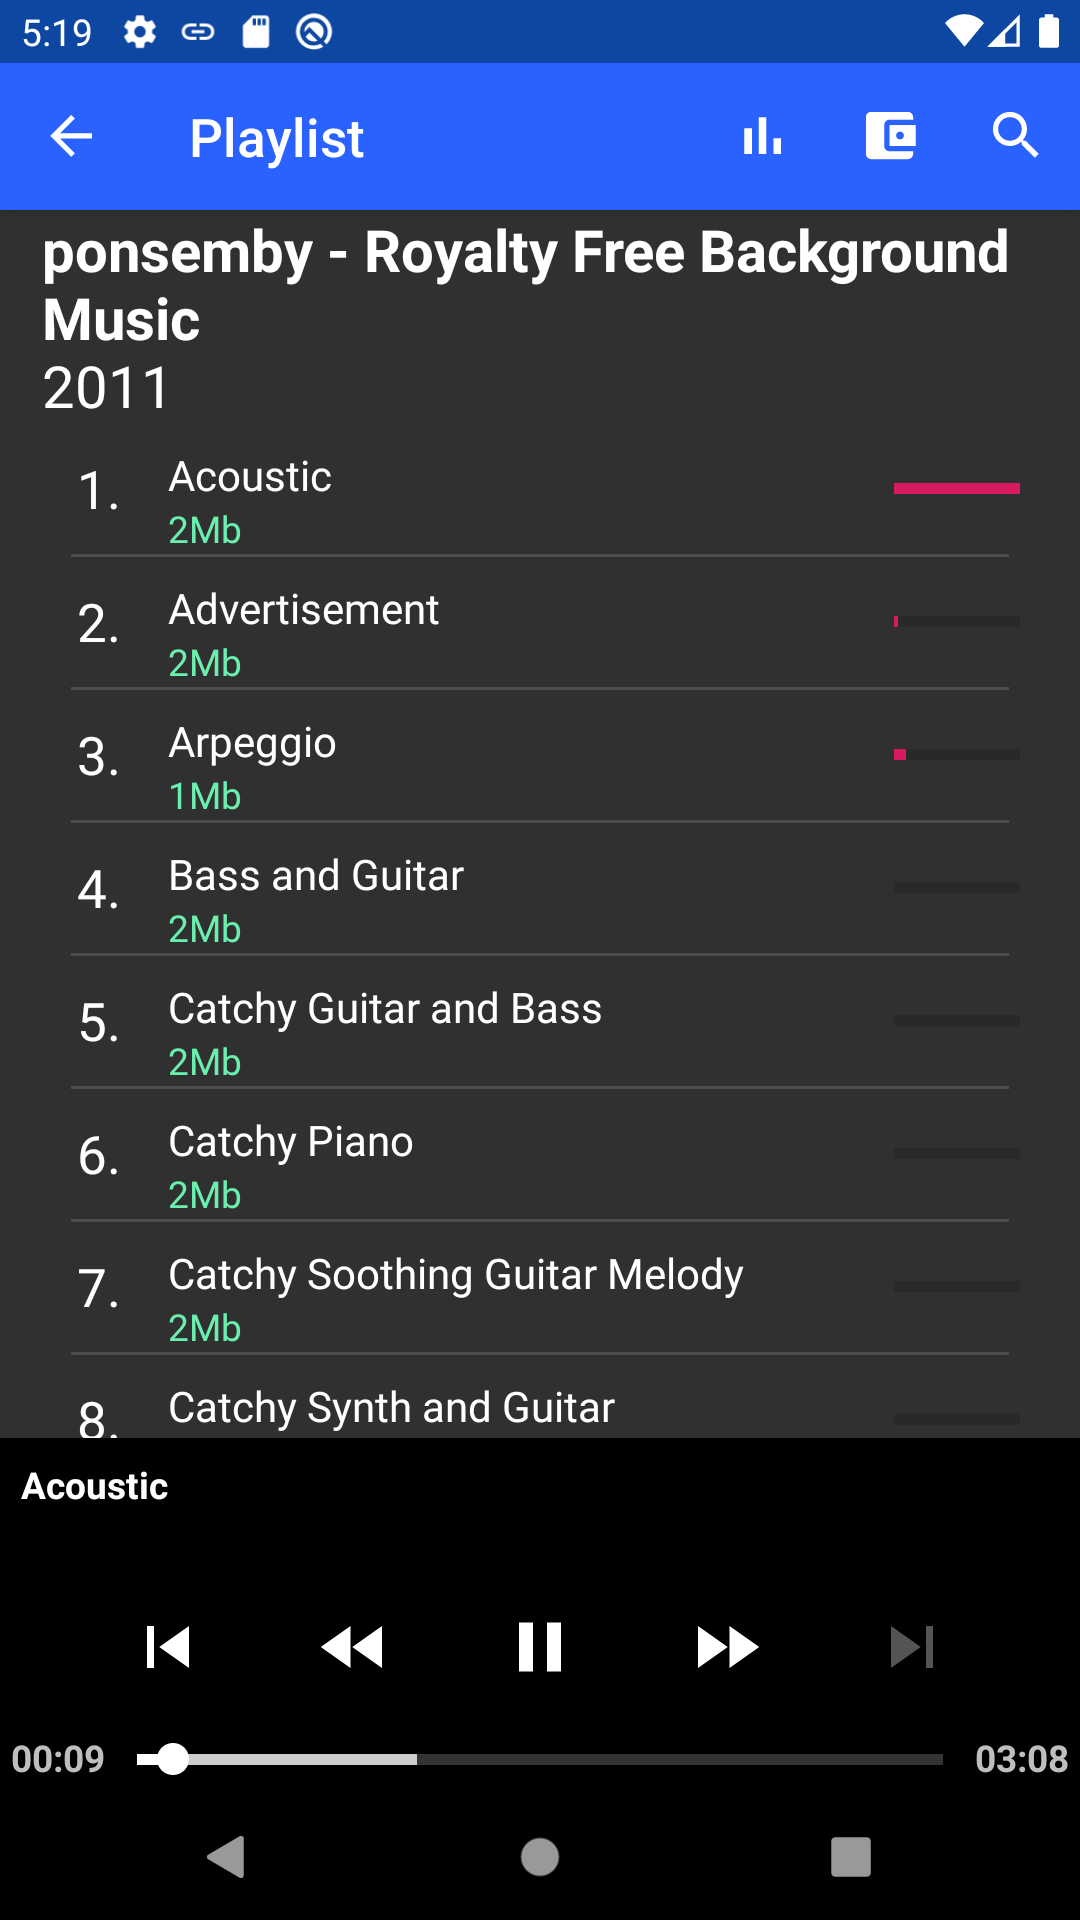
\includegraphics[width=1\linewidth]{implementation/screenshot-playlist.png}
        \caption{Playlist fragment, showing all tracks of one Release}
        \label{fig:screenshot-playlist}
    \endminipage\hfill
\end{figure}
\subsection{Playlist fragment}
A Playlist fragment interacts with exactly one Release object. The playlist fragment displays its list of tracks and other metadata, such as the title and artists of the Release (see \ref{fig:screenshot-playlist}). For each track the file size is displayed, and a loading indicator on the right side. This shows, in real time, how much of the track is downloaded. In the example of \ref{fig:screenshot-playlist}, the first track is fully loaded.
\subsection{Wallet}
Each device participating in the MusicCommunity is given a private/public wallet identity upon installation of the MusicDAO. The wallet interface (\ref{fig:wallet-sync}) shows synchronization status of the RegTest network (see \ref{sec:regtest-network-impl}). Once the wallet is fully synchronized with the blockchain, the private key and balance are displayed as shown in \ref{fig:wallet-balance}. Upon browsing a playlist, if the \textit{publisher} field is present in the corresponding Release object, a donation button is displayed as shown in \ref{fig:tip-artist}. When pressing this button, the user can select an amount and make a direct donation to the artist or band, in the form of a bitcoin transaction from their wallet. This transaction is then registered on the RegTest network.
\begin{figure}
    \minipage{0.3\textwidth}
        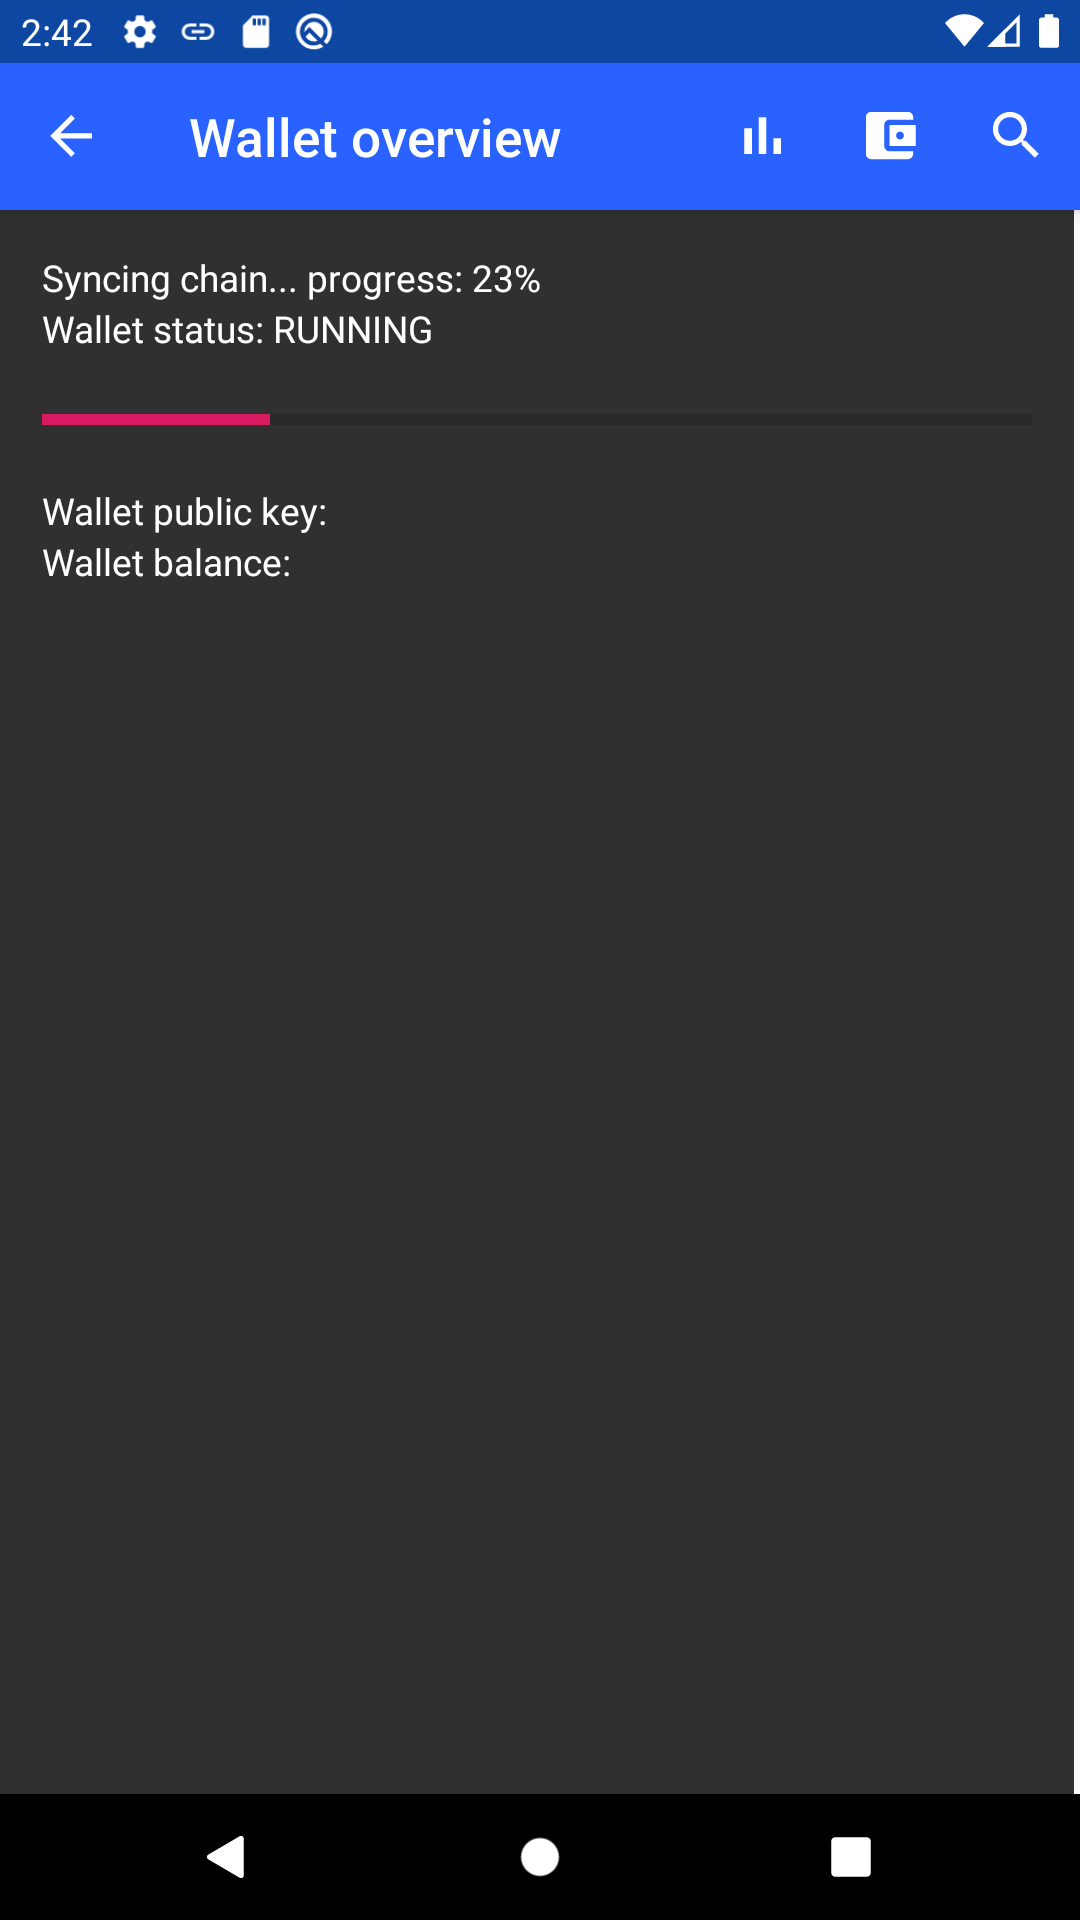
\includegraphics[width=1\linewidth]{implementation/wallet-sync.png}
        \caption{Synchronizing with the Bitcoin RegTest environment blockchain}
        \label{fig:wallet-sync}
    \endminipage\hfill
    \minipage{0.3\textwidth}
        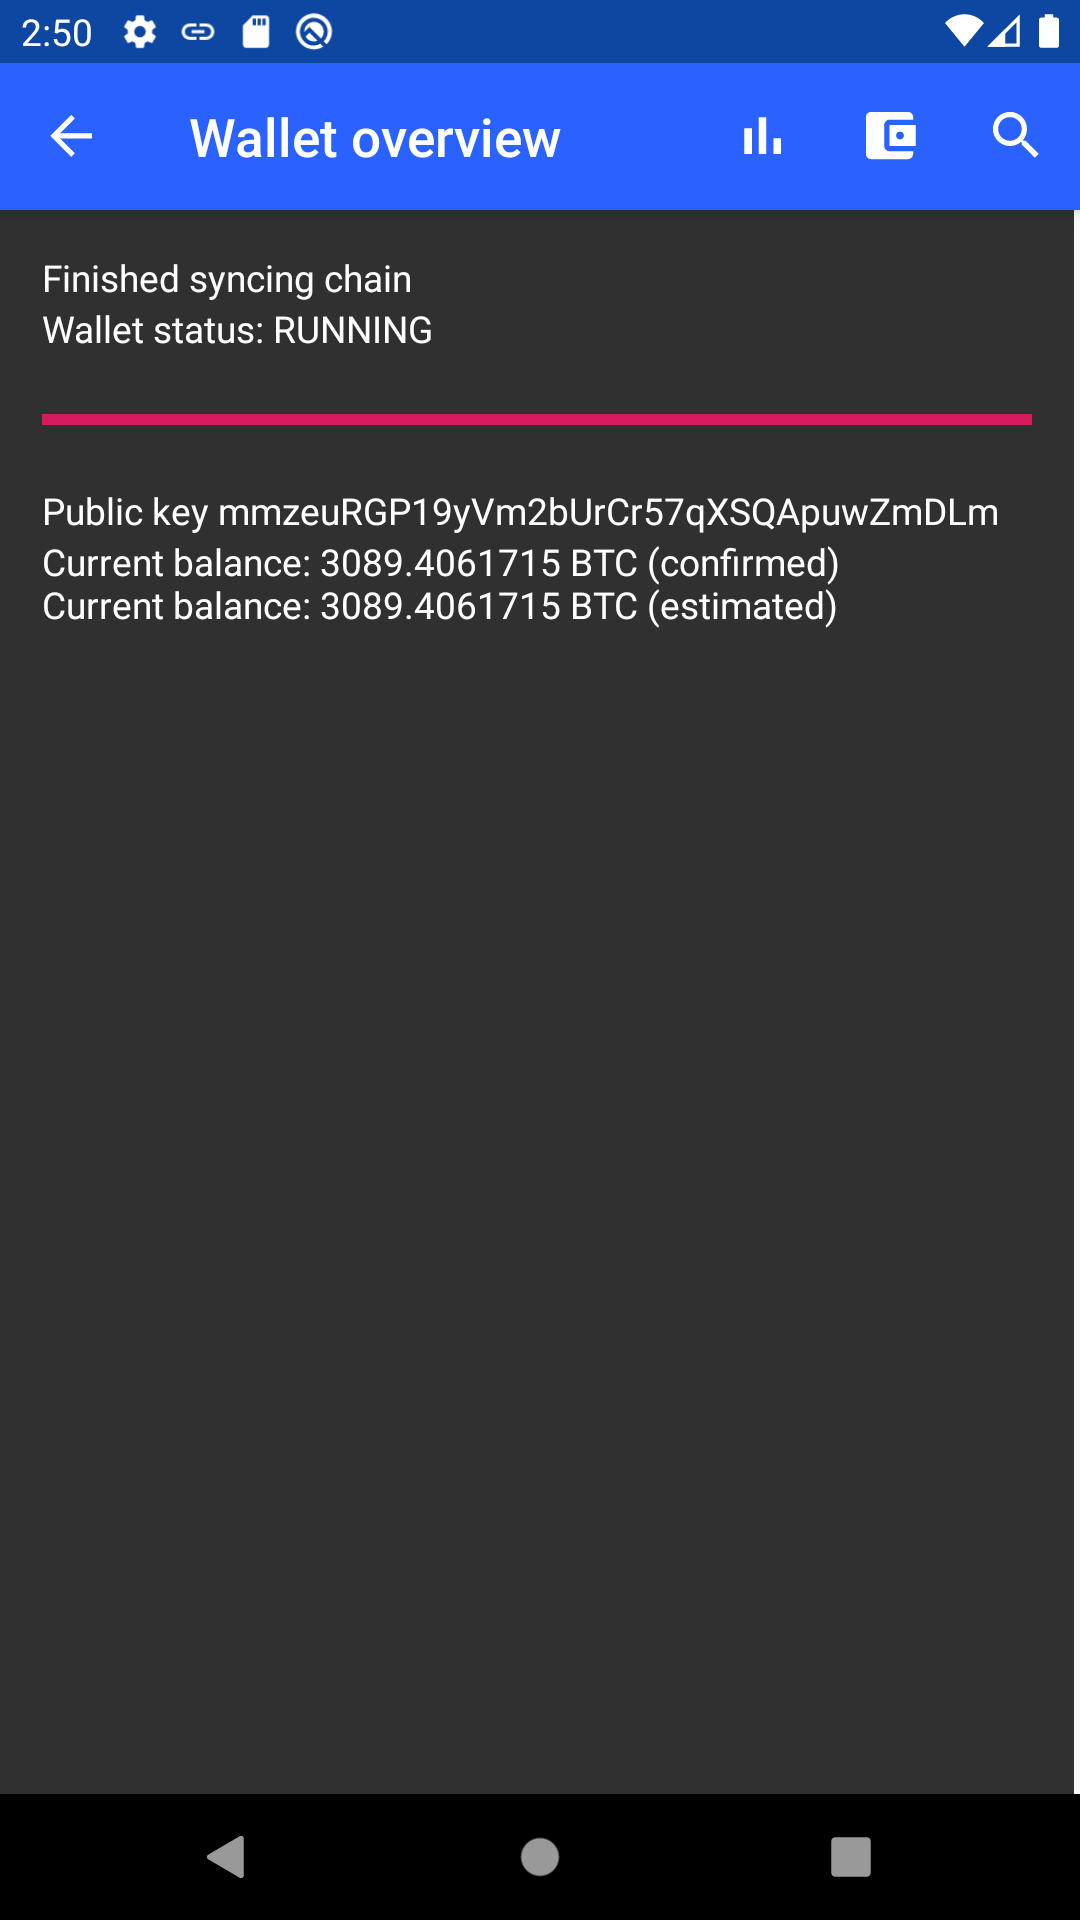
\includegraphics[width=1\linewidth]{implementation/wallet-balance.png}
        \caption{Wallet overview and balance after synchronizing}
        \label{fig:wallet-balance}
    \endminipage\hfill
    \minipage{0.3\textwidth}
        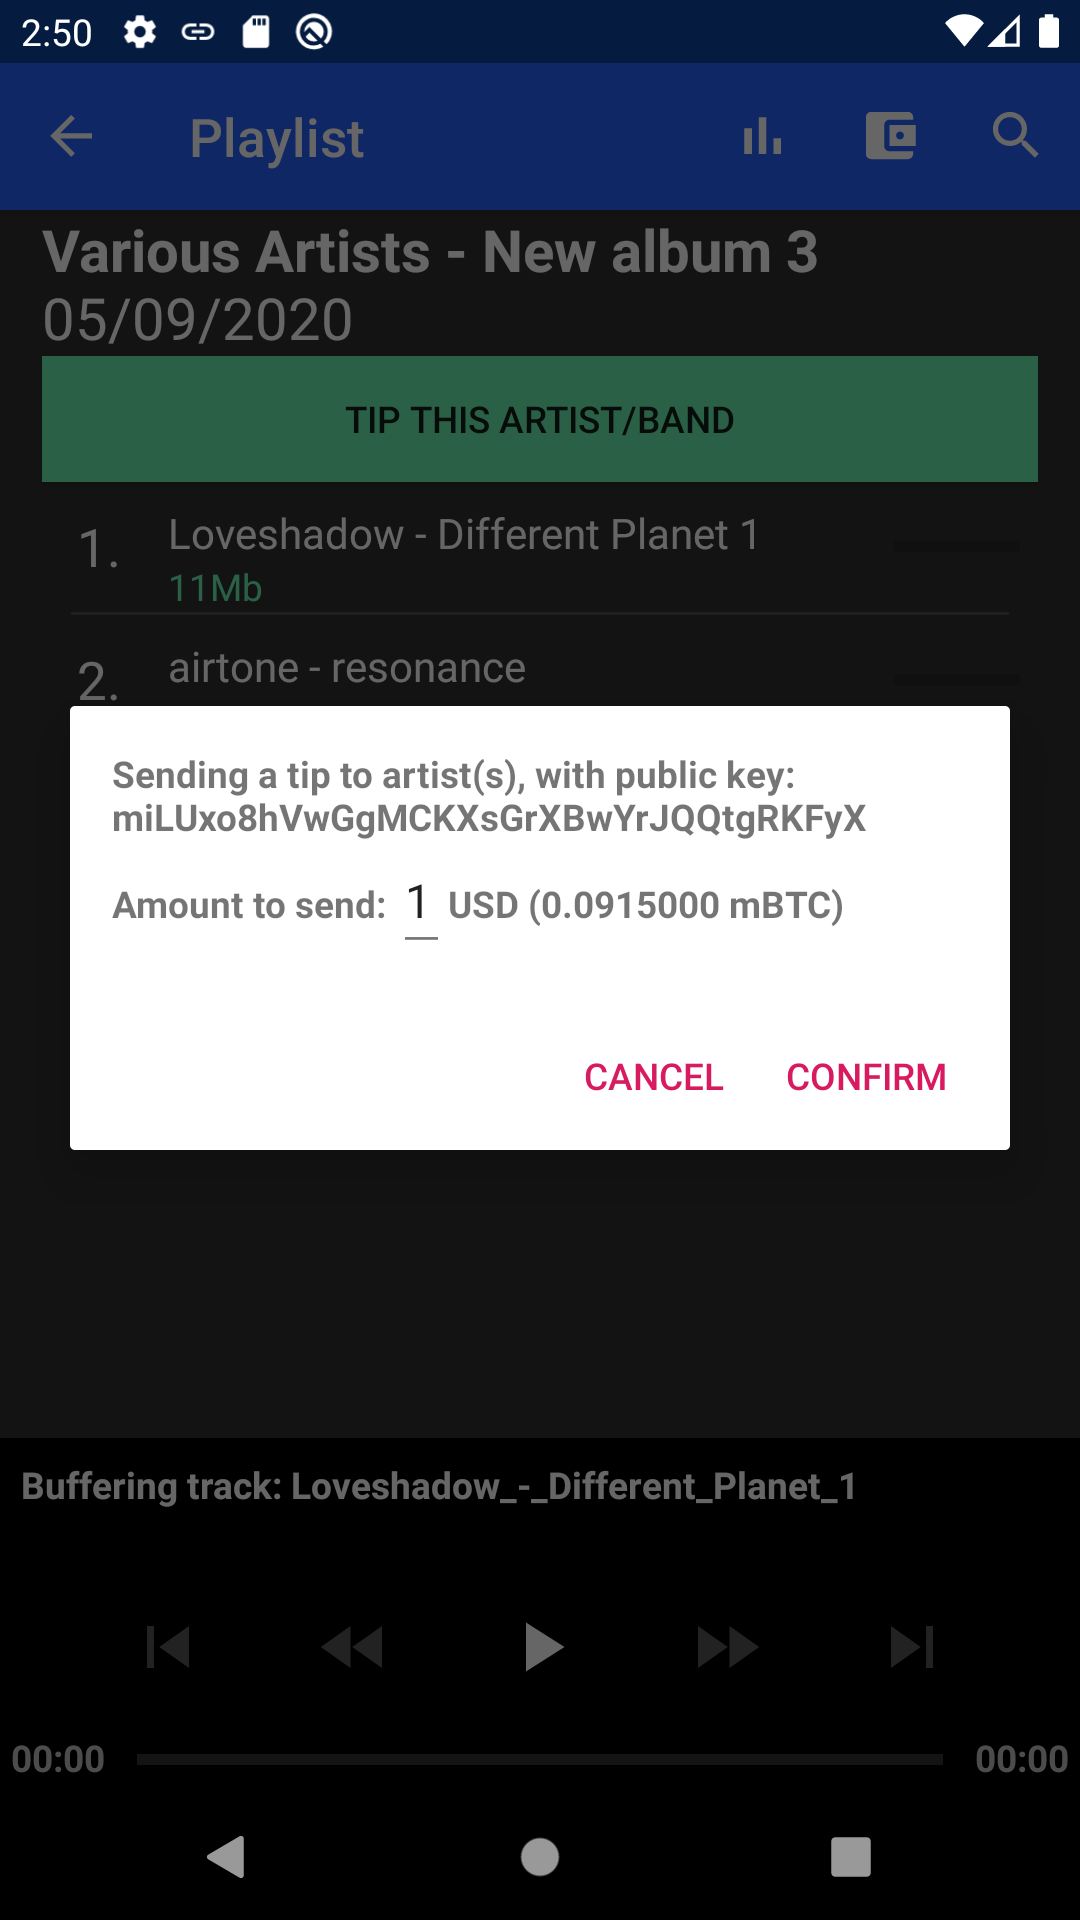
\includegraphics[width=1\linewidth]{implementation/tip-artist.png}
        \caption{Sending a tip to an artist or band}
        \label{fig:tip-artist}
    \endminipage\hfill
\end{figure}